%%%%%%%%%%%%%%%%%
% This is an example CV created using altacv.cls (v1.1, 21 November 2016) written by
% LianTze Lim (liantze@gmail.com), based on the 
% Cv created by BusinessInsider at http://www.businessinsider.my/a-sample-resume-for-marissa-mayer-2016-7/?r=US&IR=T
% 
%% It may be distributed and/or modified under the
%% conditions of the LaTeX Project Public License, either version 1.3
%% of this license or (at your option) any later version.
%% The latest version of this license is in
%%    http://www.latex-project.org/lppl.txt
%% and version 1.3 or later is part of all distributions of LaTeX
%% version 2003/12/01 or later.
%%%%%%%%%%%%%%%%

%% If you want to use \orcid or the
%% academicons icons, add "academicons"
%% to the \documentclass options. 
%% Then compile with XeLaTeX or LuaLaTeX.
% \documentclass[10pt,a4paper,academicons]{altacv}
\documentclass[10pt,a4paper]{altacv}

%% AltaCV uses the fontawesome and academicon fonts
%% and packages. 
%% See texdoc.net/pkg/fontawecome and http://texdoc.net/pkg/academicons for full list of symbols.
%% When using the "academicons" option,
%% Compile with LuaLaTeX for best results. If you
%% want to use XeLaTeX, you may need to install
%% Academicons.ttf in your operating system's font %% folder.


% Geometría de ancho completo para página 1
\geometry{left=1cm,right=1cm,top=1cm,bottom=1cm}
% Guardar geometría de dos columnas para página 2
\newcommand{\twocolgeometry}{\newgeometry{left=1cm,right=9cm,marginparwidth=6.8cm,marginparsep=1.2cm,top=1cm,bottom=1cm}}

% Change the font if you want to.

% If using pdflatex:
\usepackage[utf8]{inputenc}
\usepackage[T1]{fontenc}
\usepackage[default]{lato}
\usepackage{enumitem} % For customizing lists
\usepackage{multicol} % Para formato de múltiples columnas
\usepackage{ragged2e} % Para justificar texto
\usepackage{pgfplots} % Para gráficos de barras y radar
\usepgfplotslibrary{polar}
\pgfplotsset{compat=1.17}
% Colores para el gráfico de barras (paleta azul-verde)
\definecolor{colorB2B}{HTML}{1A5276}
\definecolor{colorProspeccion}{HTML}{1E8C8C}
\definecolor{colorCRM}{HTML}{48B4A0}
\definecolor{colorCierre}{HTML}{6BC9A6}
\definecolor{colorDificultades}{HTML}{8FD9B6}
\definecolor{colorPruebas}{HTML}{B5E7A0}

% Color coral para contraste en gráfico radar (distinto de azul/teal)
\definecolor{radarCoral}{HTML}{C97B5B}

% Colores para el wheelchart (paleta azul-teal)
\definecolor{wheel1}{HTML}{1B4F72}
\definecolor{wheel2}{HTML}{2874A6}
\definecolor{wheel3}{HTML}{1ABC9C}
\definecolor{wheel4}{HTML}{48C9B0}
\definecolor{wheel5}{HTML}{76D7C4}
\definecolor{wheel6}{HTML}{A3E4D7}

% If using xelatex or lualatex:
% \setmainfont{Lato}

% Change the colours if you want to
\definecolor{VividPurple}{HTML}{1B4A5C}
\definecolor{SlateGrey}{HTML}{2E2E2E}
\definecolor{LightGrey}{HTML}{666666}
\colorlet{heading}{VividPurple}
\colorlet{accent}{VividPurple}
\colorlet{emphasis}{SlateGrey}
\colorlet{body}{LightGrey}

% Change the bullets for itemize and rating marker
% for \cvskill if you want to
\renewcommand{\itemmarker}{{\small\textbullet}}
\renewcommand{\ratingmarker}{\faCircle}

%% sample.bib contains your publications
% \addbibresource{sample.bib} % Comentado - no se usan publicaciones

% Redefinir cvevent para que fecha y ubicación estén más juntos
\renewcommand{\cvevent}[4]{%
  {\large\bfseries\color{emphasis}#1\par}
  \smallskip
  \textbf{\color{accent}#2}\par
  \smallskip
  {\small\faCalendar \hspace{0.5em}#3\hspace{2em}%
  \ifstrequal{#4}{}{}{\faMapMarker\hspace{0.5em}#4}\par}
  \medskip
}

% Redefinir wheelchart sin centering para poder posicionarlo manualmente
\renewcommand{\wheelchart}[3]{%
    \begingroup
    \def\innerradius{#2}%
    \def\outerradius{#1}%
    \pgfmathsetmacro{\totalnum}{0}%
    \foreach \value/\colour/\name in {#3} {%
        \pgfmathparse{\value+\totalnum}%
        \global\let\totalnum=\pgfmathresult%
    }%
    \begin{tikzpicture}
      \pgfmathsetmacro{\wheelwidth}{\outerradius-\innerradius}
      \pgfmathsetmacro{\midradius}{(\outerradius+\innerradius)/2}
      \begin{scope}[rotate=-90]
      \pgfmathsetmacro{\cumnum}{0}
      \foreach \value/\width/\colour/\name in {#3} {
            \pgfmathsetmacro{\newcumnum}{\cumnum + \value/\totalnum*360}
            \pgfmathsetmacro{\percentage}{\value/\totalnum*100}
            \pgfmathsetmacro{\midangle}{-(\cumnum+\newcumnum)/2}
            \pgfmathparse{(-\midangle>180?"west":"east")} \edef\textanchor{\pgfmathresult}
            \pgfmathparse{(-\midangle>180?"flush left":"flush right")} \edef\textalign{\pgfmathresult}
            \pgfmathsetmacro\labelshiftdir{1-2*(-\midangle<180)}
            \filldraw[draw=white,fill=\colour] (-\cumnum:\outerradius) arc (-\cumnum:-(\newcumnum):\outerradius) --
            (-\newcumnum:\innerradius) arc (-\newcumnum:-(\cumnum):\innerradius) -- cycle;
            \draw [*-,thin,emphasis] node [append after command={(\midangle:\midradius pt) -- (\midangle:\outerradius + 1ex) -- (\tikzlastnode)}] at (\midangle:\outerradius + 1ex) [xshift=\labelshiftdir*0.5cm,inner sep=1ex, outer sep=0pt, text width=\width,anchor=\textanchor,align=\textalign,font=\small,text=body]{\name};
            \global\let\cumnum=\newcumnum
        }
      \end{scope}
    \end{tikzpicture}\par
    \endgroup
}

\begin{document}
\name{Ana María \newline Albarracín Noreña}
  \tagline{Ejecutiva Comercial Senior B2B}
% Cropped to square from https://en.wikipedia.org/wiki/Marissa_Mayer#/media/File:Marissa_Mayer_May_2014_(cropped).jpg, CC-BY 2.0
\photo{5.5cm}{me}
% Personal info without bullet points
\personalinfo{%
  \textcolor{accent}{\faEnvelope}\hspace{0.5em}amalbarracin5@gmail.com \\
  \textcolor{accent}{\faPhone}\hspace{0.5em}(+57) 312 825 5775 \\
  \textcolor{accent}{\faLinkedin}\hspace{0.5em}linkedin.com/in/ana-maria-albarracin \\
  \textcolor{accent}{\faMapMarker}\hspace{0.5em}Tarjeta profesional: 26272
}

\makecvheader

\cvsection{Perfil}
{\small\justifying
Ejecutiva Comercial Senior B2B con sólida formación técnica y enfoque en ventas consultivas para cuentas claves.\\
Experiencia en negociación B2B, soporte técnico y desarrollo de mercado en energías renovables y químicos especializados (polímeros).\\
Logros: 125\% de cumplimiento del presupuesto anual; ascenso a Líder/Especialista de Línea.
\par}

\cvsection{Experiencia Laboral}
\cvevent{Ejecutiva Comercial Senior - Especialista de Línea}{Meico Solar}{Mayo 2024--Actualidad}{Bogotá, Colombia}
{\color{accent}\textbf{Ascenso: Ejecutiva Comercial Senior - Especialista de Línea}} {\small\textit{(Octubre 2025)}}
\begin{itemize}
\item Gestión de cuentas clave y liderazgo en negociaciones estratégicas de línea de producto.
\item Capacitación y mentoría al equipo comercial; seguimiento y control del presupuesto de línea.
\item Elaboración y seguimiento de estrategias comerciales; gestión de presupuestos y forecast de ventas.
\item Gestión de relaciones con proveedores; negociación de precios y asignación de presupuesto para actividades de mercadeo.
\end{itemize}

{\color{accent}\textbf{Ejecutiva Comercial}}
\begin{itemize}
\item Gestión comercial integral: prospección, identificación de necesidades, cotización, seguimiento estratégico y cierre de ventas con acompañamiento postventa.
\item Experiencia en ventas B2B con empresas del sector energético; capacidad de adaptación para operaciones con clientes internacionales.
\item Realización de visitas de relacionamiento en Bogotá y el Eje Cafetero para fortalecer vínculos con clientes actuales y potenciales.
\item Análisis del mercado y mantenimiento del CRM para identificar oportunidades comerciales.
\end{itemize}

\vspace{0.2 cm}
\cvevent{Asesora Técnica Comercial - Coordinadora de Exportaciones}{Olaflex SAS}{Julio 2022--Mayo 2024}{Bogotá, Colombia}

\begin{itemize}
\item \textbf{Coordinación de exportaciones:} Gestión integral del proceso de exportación de productos de poliuretano a mercados internacionales, desde la cotización hasta la entrega.
\item \textbf{Documentación aduanera y legal:} Elaboración y tramitación de documentación para embarques: facturas comerciales, certificados de origen, listas de empaque, documentos de transporte y cumplimiento de normativas aduaneras.
\item Gestión de ventas B2B con clientes nacionales e internacionales, incluyendo visitas, seguimiento y soporte técnico en planta.
\item Propuesta de desarrollos a medida según el uso final del cliente, pruebas de desempeño y formulación de soluciones personalizadas para mercados de exportación.
\item Elaboración de planes de marketing y proyección de presupuestos para líneas de producto con potencial exportador.
\end{itemize}

\cvevent{Asesora Comercial}{Química MG}{Enero 2022--Julio 2022}{Bogotá, Colombia}

\begin{itemize}
\item Participación en licitaciones y proyectos de ingeniería con alcance nacional e internacional.
\item Elaboración de propuestas comerciales y seguimiento a clientes.
\end{itemize}

\cvevent{Gestora de Proyectos}{Grupo Coral SAS}{Enero 2020--Agosto 2021}{Bogotá, Colombia}

\begin{itemize}
\item Elaboración de propuestas técnico-comerciales para clientes del sector público y privado.
\item Apoyo en procesos licitatorios y desarrollo de nuevos negocios.
\end{itemize}

% Inicio de sección en dos columnas
\begin{multicols}{2}

\vspace{1.0CM}
\cvsection{¿Qué información obtengo en una reunión comercial?}
\vspace{-2.3CM}
{\small\justifying En una reunión con el cliente, mediante las preguntas adecuadas, identifico la siguiente información clave:\par}
\vspace{0.2cm}
\noindent\makebox[\columnwidth][l]{%
\hspace{-3cm}\wheelchart{2.5cm}{0.5cm}{%
25/12em/wheel1/Conocimiento\\del cliente,
20/12em/wheel2/Competencia,
20/12em/wheel3/Propuesta\\comercial,
20/12em/wheel4/Estado de\\negociación,
15/12em/wheel5/Conocimiento\\del negocio}}

\vspace{0.3cm}
{\small\justifying
\textbf{\color{accent}Conocimiento del cliente:} Necesidades, objetivos, estructura de decisión y pain points.\\[2pt]
\textbf{\color{accent}Competencia:} Proveedores actuales, alternativas consideradas y puntos de diferenciación.\\[2pt]
\textbf{\color{accent}Propuesta comercial:} Alcance, timing, condiciones y valor percibido de la oferta.\\[2pt]
\textbf{\color{accent}Estado de negociación:} Etapa del proceso, próximos pasos y criterios de decisión.\\[2pt]
\textbf{\color{accent}Conocimiento del negocio:} Industria, procesos, tendencias y contexto del comprador.\par
}
\vspace{-3.5cm}
\cvsection{Referencias}
\vspace{-2.2cm}
{\small
\noindent\textbf{\color{emphasis}Daniela Perdomo Morales}, Ejecutiva comercial, Biopolar\\
\textcolor{accent}{\faPhone}\hspace{0.5em}+57 313 8653659\par
\vspace{0.25cm}
\noindent\textbf{\color{emphasis}Juan David Tuta Botero}, Líder de ingeniería, Unosquare\\
\textcolor{accent}{\faPhone}\hspace{0.5em}+57 3016395759\par
}

\columnbreak

\vspace{1.2cm}
\cvsection{Habilidades Comerciales}
\begin{center}
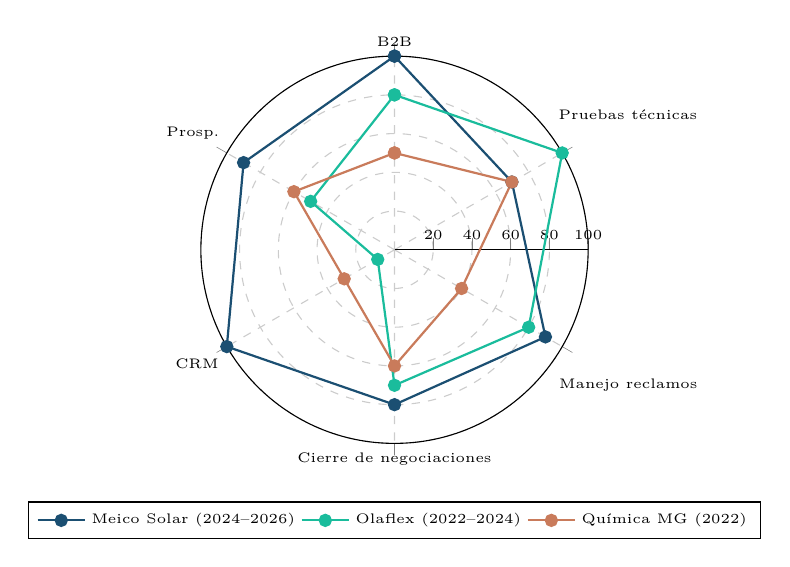
\begin{tikzpicture}
\begin{polaraxis}[
    width=6.5cm,
    height=6.5cm,
    grid=both,
    major grid style={dashed, gray!40},
    minor grid style={dashed, gray!20},
    xtick={90,150,210,270,330,30},
    xticklabels={B2B, Prosp., CRM, Cierre de negociaciones, Manejo reclamos, Pruebas técnicas},
    xticklabel style={font=\tiny},
    ytick={20,40,60,80,100},
    yticklabels={20,40,60,80,100},
    yticklabel style={font=\tiny},
    ymin=0, ymax=100,
    legend style={
        at={(0.5,-0.15)},
        anchor=north,
        legend columns=3,
        font=\tiny
    },
]
\addplot+[draw=wheel1, mark=*, thick, mark options={fill=wheel1, draw=wheel1}] coordinates {
    (90,100) (150,90) (210,100) (270,80) (330,90) (30,70) (90,100)
};
\addlegendentry{Meico Solar (2024--2026)}
\addplot+[draw=wheel3, mark=*, thick, mark options={fill=wheel3, draw=wheel3}] coordinates {
    (90,80) (150,50) (210,10) (270,70) (330,80) (30,100) (90,80)
};
\addlegendentry{Olaflex (2022--2024)}
\addplot+[draw=radarCoral, mark=*, thick, mark options={fill=radarCoral, draw=radarCoral}] coordinates {
    (90,50) (150,60) (210,30) (270,60) (330,40) (30,70) (90,50)
};
\addlegendentry{Química MG (2022)}
\end{polaraxis}
\end{tikzpicture}
\end{center}

\vspace{0.2cm}
{\small\justifying
\textbf{\color{accent}B2B:} Negociación con empresas.\\
\textbf{\color{accent}Prospección:} Búsqueda, contacto, presentación de la empresa y calificación de clientes potenciales.\\
\textbf{\color{accent}CRM:} Registro de negocios, seguimiento oportuno y gestión del proceso comercial.\\
\textbf{\color{accent}Cierre:} Negociación final y cierre efectivo de ventas.\\
\textbf{\color{accent}Manejo de reclamos:} Gestión de clientes inconformes e incidencias.\\
\textbf{\color{accent}Pruebas técnicas:} Capacitación de personal y pruebas de funcionamiento del material en diferentes ambientes de producción.\par
}

\vspace{-0.2cm}
\cvsection{Educación}
\vspace{-0.3cm}
\cvevent{Maestría en Ingeniería Química}{Universidad Nacional de Colombia}{2023--Actualidad}{Bogotá, Colombia}
{\justifying Trabajo de grado en curso: Comparación de métodos multicriterio para la selección de tecnologías de captura y aplicación de CO en industrias de alta contribución de emisiones. El proyecto integra tecnologías como absorción con aminas, membranas y adsorción en sólidos, evaluadas mediante herramientas como AHP, TOPSIS y Fuzzy TOPSIS.\par}

\vspace{0.4cm}
\cvevent{Ingeniería Química}{Universidad Nacional de Colombia}{2013--2019}{Bogotá, Colombia}
{\justifying Trabajo de grado: Comparación de catalizadores para la hidrólisis de plasma con fines alimenticios. Formación sólida en procesos químicos, control de calidad y análisis fisicoquímico. Experiencia práctica en la industria de fragancias, incluyendo muestreo, SAP y liberación de lotes.\par}

\end{multicols}

\end{document}
